\section{Laboratory work implementation}

\subsection{Tasks and Points}

\begin{itemize}
	\item Advanced Level (nota 9 || 10):
	\begin{itemize}
		\item Realizeaza o aplicatie care va implimenta tehnica Pomodoro
	\end{itemize}
\end{itemize}

\subsection{Analiza lucrarii de laborator}

Am dezvoltat o apicatie Android in IDE-ul AndroidStudio, proiectul cnstruit pe un empty activity.
Primul activity MainActivity este legat cu layout-ul actity care contine partea grafica ferestrei si arata astfel:


\begin{center}
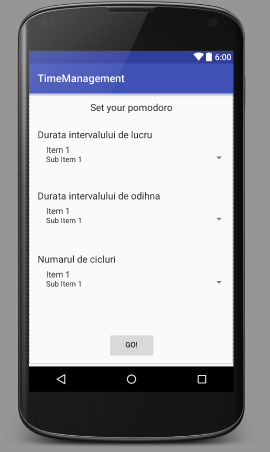
\includegraphics[width=0.3\linewidth]{img1}
\end{center}

Acesta contine 4 text-formuri, cu informatie, 3 drop-downuri cu posibilitatea de selectare din resursele strings.xml si un buton care ne trimite la layout-ul timer, acela fiind legat cu TimeActivity. Asa arata structura proiectului:

\begin{center}
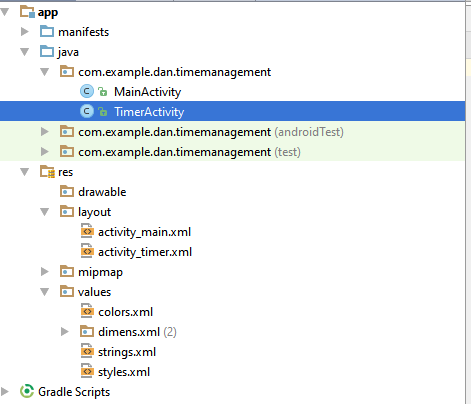
\includegraphics[width=0.5\linewidth]{img2}
\end{center}

Layout-ul timer-ului arata astfel:
\begin{center}
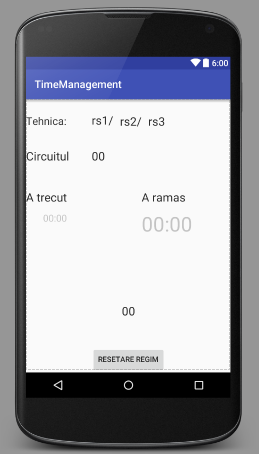
\includegraphics[width=0.4\linewidth]{img3}
\end{center}

Acesta contine texte infomrative, label-urile rs1, rs2, rs3 sunt intent.PutExtra din transmise din primul activity si afisate aici, Circuitul reprezinta iteratia facuta de program, 2 timer-uri, dintre care doar unul este pornit, ne afiseaza cit timp a trecut de la onCreate, si al 2-lea ne afiseaza cit timp a ramas pina la intrerupere. Textul de jos ne indica actiunea pe care trebuie sa o facem la moment, si un buton care ne intoarce la MainActivity(cel precedent).
Asa arata rularea primei ferestre:
\begin{center}
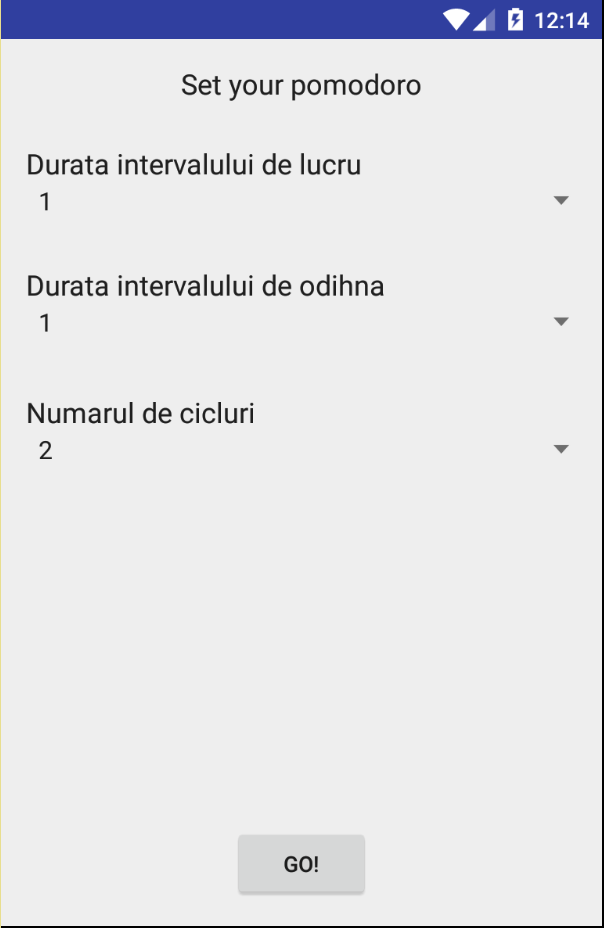
\includegraphics[width=0.4\linewidth]{img4}
\end{center}
Observam posibilitatea de alegerea duratei de timp pentru pomodor, durata de timp pentru odihna si numarul de circuite acestei configuratii. Acest dropdown arata astfel:
\begin{center}
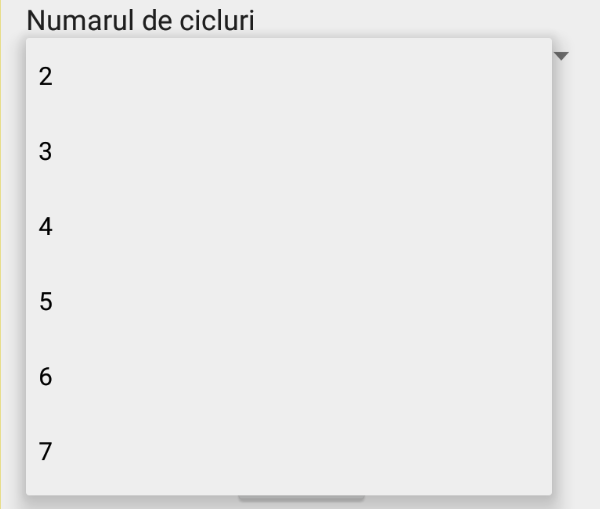
\includegraphics[width=0.3\linewidth]{img5}
\end{center}
La apasarea butonului trecem la timer activitity care in functionare arata astfel:
\begin{center}
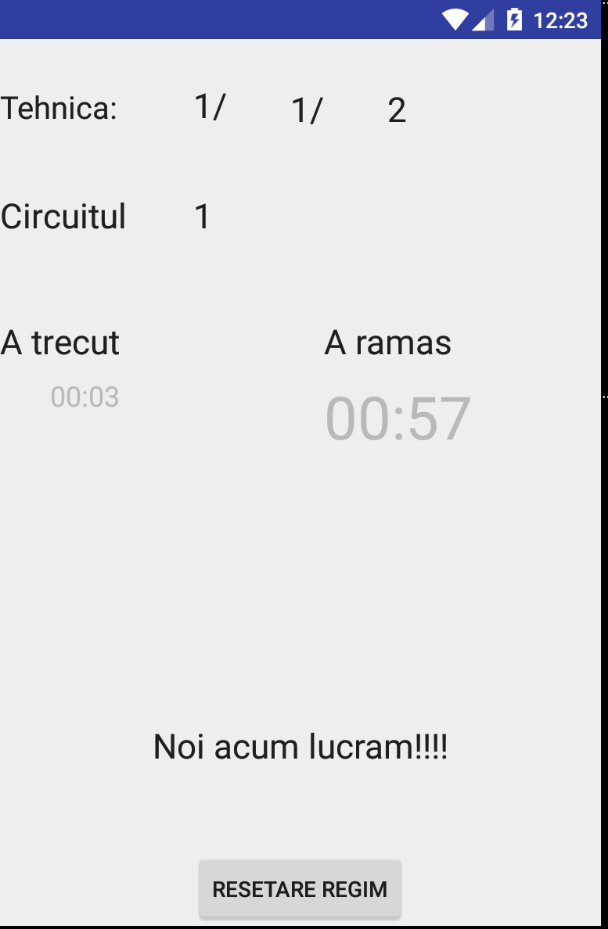
\includegraphics[width=0.3\linewidth]{img6}
\end{center}
In cind timer-ul ajunge la valoarea necesara, apare dialog-boxul cu o optiunea de continuare:
\begin{center}

\includegraphics[width=0.4\linewidth]{img7}
\end{center}
Dupa tastarea butonului, se afiseaza un text de dialog cu utilizatorul si este rulata urmatoarea etapa a timer-ului 
\begin{center}

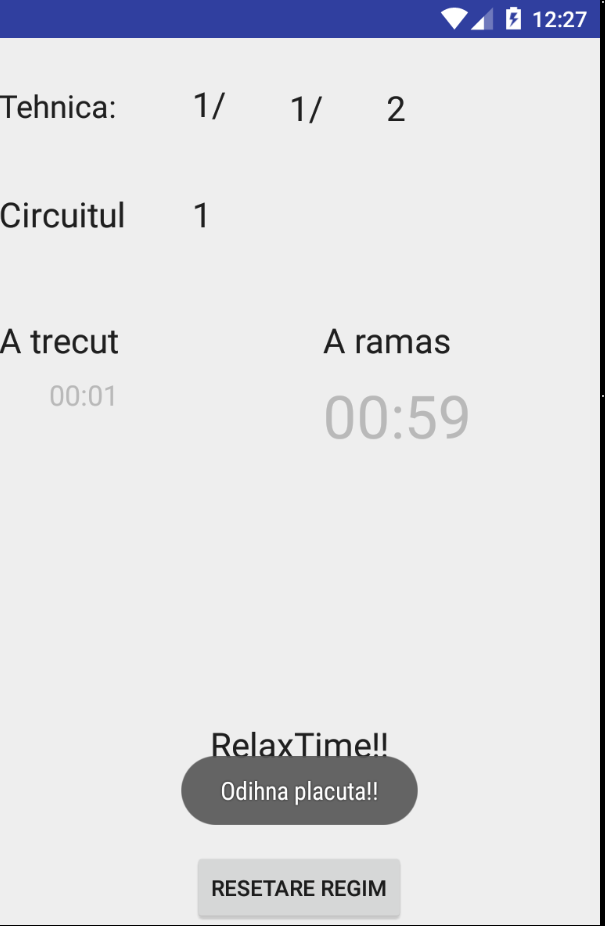
\includegraphics[width=0.4\linewidth]{img8}

\end{center}
Paralel, in cazul in care programul este in background, primim o notificare cu sunet permanent pe care in cazul inchiderii, la fel, trecem la urmatoarea etapa. Aceasta notificare arata astfel:
\begin{center}
\centering
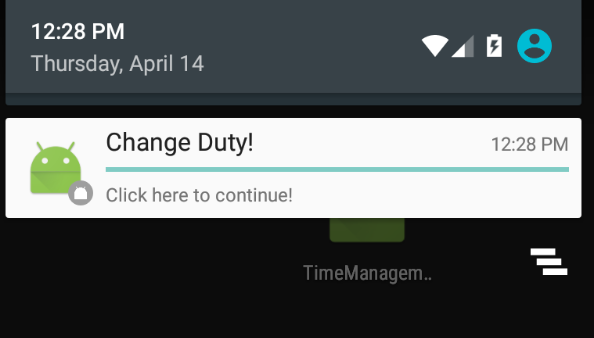
\includegraphics[width=0.7\linewidth]{img9}
\caption{}
\label{fig:img9}
\end{center}
In momentul in care a trecut o etapa de lucru si una de odihna, acesta trece la urmatoarea iteratie care la fel incepe cu etapa de lucru:
\begin{center}
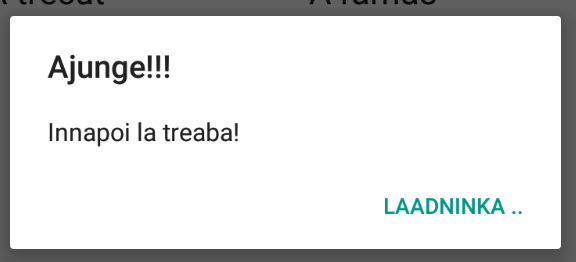
\includegraphics[width=0.4\linewidth]{img10}
\end{center}
Si afisarea urmatorului pas:
\begin{center}
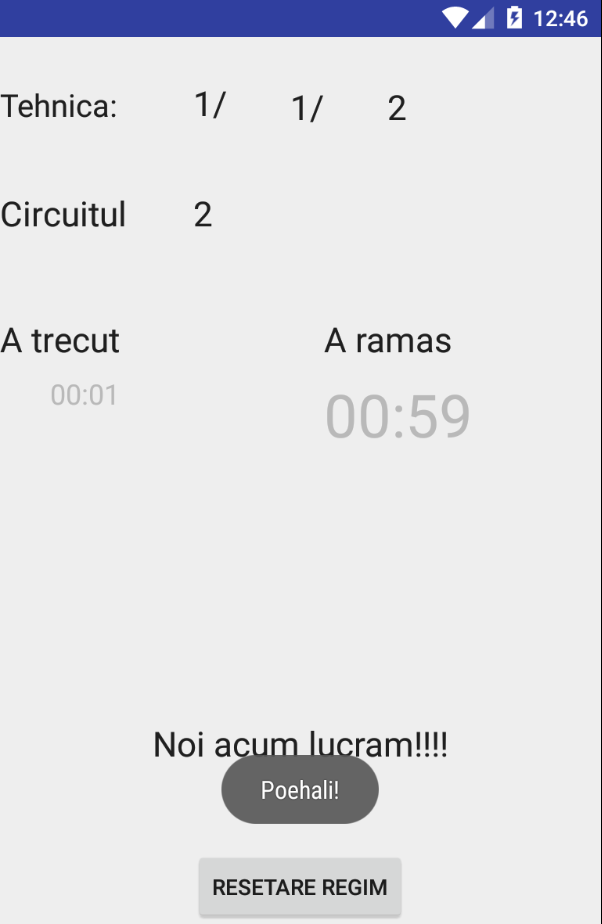
\includegraphics[width=0.4\linewidth]{img13}
\end{center}

Dupa care se repeta aceste actiuni pina la completarea tuturor iteratiilor setate anterior, dupa care textul ce ne indica actiunea ne arata ca Pomodoro sa terminat:
\begin{center}
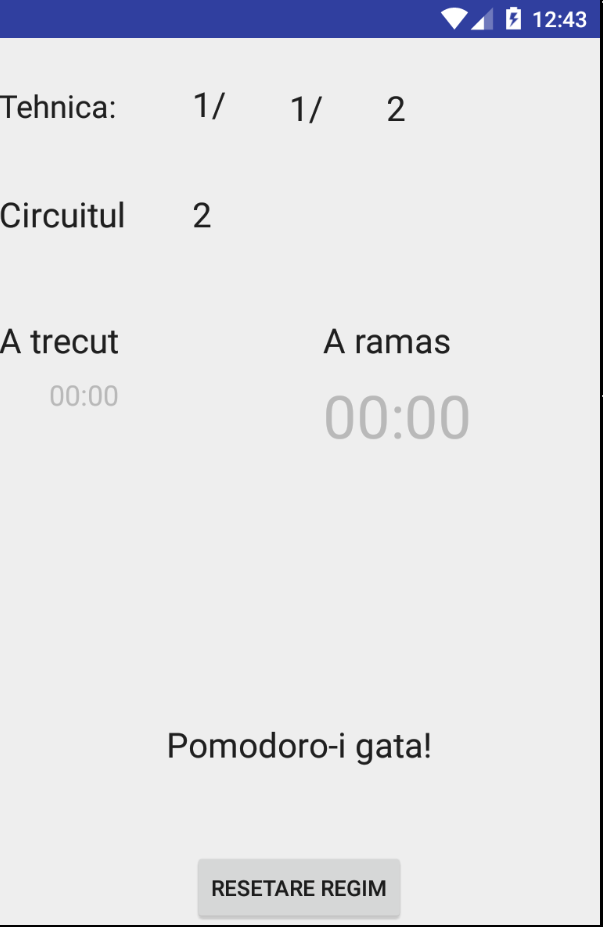
\includegraphics[width=0.4\linewidth]{img12}
\end{center}
Putem tasta butonul resetarii regimului pentru o configurare noua a timer-ului din primul activity cu afisarea layout-ului main.



\clearpage



